

\vspace{-2mm}
\section{Introduction}
\vspace{-1mm}

% Scaling laws are English-Centric. Multilingual SCLs are limited.
Scaling laws research has focused overwhelmingly on English \citep{kaplan2020scaling, hoffmann2022training, li2025mis}.
However, most of the major closed and open models now explicitly target massively multilingual uses \citep{openai2025gpt5, claude4, deepmind2025gemini25deepthink, deepseekv3, olmo2}.
Nonetheless, multilingual scaling laws research in the public sphere is limited.
Among proprietary lab reports, only Llama-3 briefly discuss their multilingual scaling laws, though they train on only 8\% non-English tokens \citep{dubey2024llama}.
Prominent public work investigates scaling laws for data mixing \citep{goyal2024scaling, ye2024data, ge2024bimix}, scaling laws for machine translation
\citep{fernandes2023scaling, gordon2021data}, multilingual instruction tuning/adaptation \citep{shaham2024multilingual, lai2024llms, weber2024investigating}, and only a couple of recent rigorous contributions investigate scaling for smaller multilingual models (<$45M$ and <$1.2B$ respectively) \citep{chang2024multilinguality, he2024scaling}.

% Our research questions, setup, and scope of experimentation.
Extending these prior works, we seek to fill the ample remaining knowledge gaps with comprehensive examinations of the following research questions.
First, we explore how the properties of different languages' scaling laws differ.
Second, we measure the cross-lingual transfer benefits between 38 languages.
To our knowledge, this represents the most comprehensive available empirical resource to explicitly measure language transfer across $38 \times 38 = 1444$ language pairs.
Third, we succeed in modeling the \emph{curse of multilinguality}---the phenomena where adding languages to the training mixture can degrade loss for each language, due to limited model capacity.
Lastly, we measure when it is more efficient to pretrain from scratch, or finetune from a general-purpose multilingual checkpoint, resolving an unaddressed practical question.
In pursuing these research questions, we develop new tools and estimates for multilingual practitioners, as well as the \ourscl{}, which significantly outperforms prior work across several dimensions of generalization.
In total, our pretraining and finetuning experiments span $774$ independent experiments on MADLAD-400 \citep{kudugunta2024madlad}, for models sized $10M-2B$, and evaluating 48 languages.
Our main contributions include:
% \vspace{-2mm}
\begin{enumerate}
    \item \textbf{The \ourscl{}} that offers better multilingual generalization to larger/unseen $N,D,C,$ and training mixes $M$, than prior work (\Cref{tab:evaluations}). In \Cref{fig:monolingual-scaling} we also estimate a compute efficiency tax between multilingual and monolingual training.
    \item \textbf{A $38 \times 38$ \textsc{Cross-Lingual Transfer Matrix}}, providing the largest resource for empirically measured transfer benefits/interference between languages (\Cref{fig:language-transfer-heatmap}).
    \item \textbf{A scaling law for the \emph{curse of multilinguality}}, that informs practitioners how much to scale $(N,D)$ to accommodate expansions in a models' language coverage (\Cref{fig:capacity_add_lang_isoloss_curve}).
    \item \textbf{A general pretrain vs finetune formula}, that informs practitioners whether it is more efficient to pretrain from scratch or begin from a multilingual \unimax{} checkpoint (\Cref{fig:modelsize_vs_finetune_intersection}).
\end{enumerate}


\begin{figure*}[t]
    \centering
    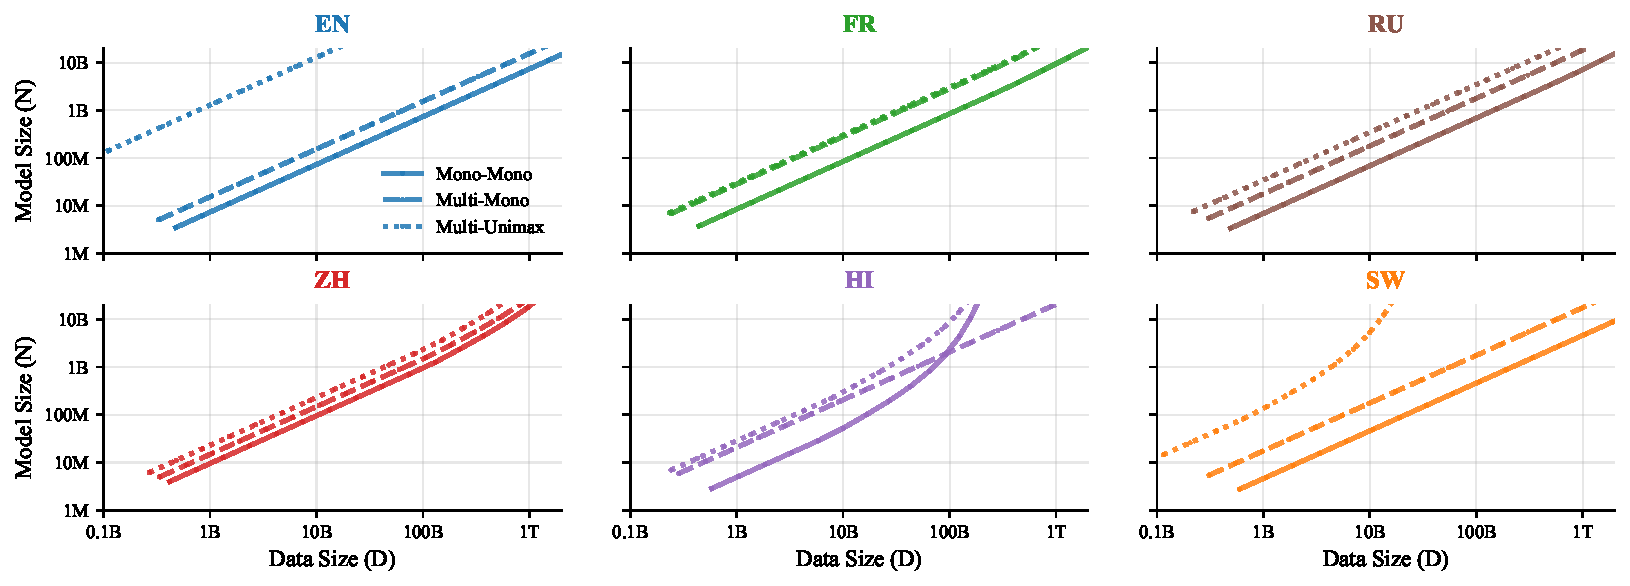
\includegraphics[width=\textwidth]{figures/scaling-laws/monolingual-scaling.pdf}
    \caption{
        \textbf{Optimal Scaling Trajectories} for English, French, Russian, Chinese, Hindi, and Swahili.
        The law for [monolingual vocabulary, monolingual training]=(\textbf{---}), the law for [multilingual vocabulary, monolingual training]=(\textbf{- - -}), and the law for [multilingual vocabulary, unimax training]=(\textbf{···}).
        \textbf{We find (1) per-language optimal scaling trajectories are similar, (2) there is a compute efficiency tax for training with \emph{multilingual} vocabularies or training sets (especially for English), and (3) as Hindi and Swahili observe data repetition their curves slope upward from diminishing returns.}
    }
    \label{fig:monolingual-scaling}
    % \vspace{-4mm}
\end{figure*}

% Our contributions
% 1. Unified Scaling Law for monolingual and multilingual settings. --> More robust and SOTA.
% 2. 30x30 language-transfer matrix
% 3. curse of multilinguality, capacity constraints, K to K+1
% 4. pretrain vs finetune.





% Large scale foundation models \citep{bommasani2021opportunities} are often English-centric \citet{reid2024gemini,openai2023gpt,team2024gemma}, with minimal amounts of data in low resource languages, if any. Foundation models that seek to support more languages tend to (a) co-train all languages in a single model \citep{leong-etal-2022-bloom,kudugunta2024madlad,dang2024aya} or (b) fine-tune a foundation model trained on primarily English \citep{tejaswi2024exploring} or other high resource languages \citep{bapna-etal-2022-building} using data in the target language. However, it is not clear if any of these choices are optimal, and would lead to the best foundation models possible for a given language. We propose using scaling laws \citep{kaplan2020scaling} to scrutinize this decision. That is, we will extrapolate the optimal architecture and hyper parameters settings from smaller training runs by describing the relationship between loss, or task performance, and scale. While there are several tools researchers have used to study the relationship between the optimal data mixture for training foundation models and scale (See Section \ref{sec:rw}), these studies are not suitable for studying foundation models that support under-resourced languages. We propose empirically demonstrating these deficiencies, and developing a theory of scaling that enables to us to study the best practices for developing models that work well for low-resource languages. More concretely, we seek to develop analytical tools for predicting scaling laws for low-resource language that:

% \begin{itemize}
%     \item Consider data constrained languages.
%     \item Consider data repetitions.
%     \item Consider large, uneven data mixtures.
% \end{itemize}


% % Currently, the status quo for training large language models (LLM) in languages other than English is training as many languages as possible in 1 model, or trying to adapt a model that is already trained to new languages. Intuitively, these are not optimal ways to train a language model that is as high quality as possible for a specific language. That is, in practice, getting LLMs to support lower-resourced languages is an afterthought in model development. We propose using scaling laws to carefully study this problem, and provide recommendations to practitioners on the optimal way to obtain good quality for a given language. We plan to go beyond the resource-rich assumption that previous works make, given that many languages have limited dataset sizes.

% For the scope of this project, we seek to find the optimal amount of data to use and the correct stage of model development at which to add data. That is, we ask the following research questions: 

% \begin{itemize}
%     \item How do scaling laws vary for different MADLAD-400 language models?
%     \item Under language capacity constraints, how will adding other language data create constructive or destructive interference? Can we predict this interference? Does this interference align with language families, scripts, or other generalizable linguistic concepts?
%     \item Can we derive laws for “multilingual plasticity” – i.e. measure how much pretraining accelerates learning for a single language in post-training vs can pretraining hurt (or “ossify”) performance for small models if it is too distinct from the post-training language?
% \end{itemize}

% In this project, our contributions are as follows:
% \begin{itemize}
%     \item We find that the optimal tokens to model size ratio varies significantly by language, as prepared in MADLAD-400---some languages may need to be trained for significantly longer than English datasets for optimal use of training compute budget. 
%     \item Then, we empirically examine the compute overhead/efficiency associated with achieving the same quality when training a bilingual model compared to a monolingual model.
%     \item Based on these results, we provide recommendations for reducing the training and inference costs for high quality multilingual models.
% \end{itemize}

% \subsection{Societal Implications}

% \paragraph{Better Multilingual Models} Over half of all content on the internet is in English - this is reflected in the prioritization of English in the creation of most frontier models \citep{openai2023gpt,reid2024gemini,team2024gemma,dubey2024llama}, with the inclusion of some amount of multilingual data,. While some high resource languages such as Mandarin or French have extremely large datasets available, and are often included in training datasets for these models, many languages have little or no data available \citep{joshi2020state}. We note that some open source multilingual models do exist \citep{ustun2024aya,kudugunta2024madlad} - however, the optimal method of obtaining high quality performance for a language with limited data is understudied. Better quality language tools in other languages has social good for purposes such as disseminating COVID-19 information during the pandemic \citep{mukhija2021designing}, internationalizing job advertisements \citep{gonzalez2023beyond,somers1997multilingual}, disseminating news during political instability \citep{haroutunian2022ethical}  or platform moderation.
% % Different languages have different fates. frontier models do not have prioritization, just a few languages. some open source models highly multilingual.  
% This work will enable the development of better tool in low-resource languages, bridging the gap in capabilities of foundation models between low-resource languages and English.

% \paragraph{Energy Consumption of Large Multilingual Models} In deep learning, it has been shown over and over again \citep{sutton2019bitter} that the most effective way of training better models has been leveraging larger amounts of compute. Foundation models are also similar, with the scale of SOTA (state-of-the-art) models increasing significantly over the last few years. Moreover, scaling up models can even introduce new abilities that previously did not exist in smaller models, which can unlock even more applications for foundation models \citep{wei2022emergent}. 

% However, scaling up these models involves significant increases in energy consumption via GPU or TPUs. For example, Llama 3 \citep{dubey2024llama} uses 16,000 GPUs  for training and 8-GPUs for serving. During training, models also use CPU resources and access main memory, which also use a significant amount of energy. 

% Meta reports the carbon emissions of the largest Llama 3 model: on using 16k H100 GPUs for $\approx 80$ days with a $40\%$ utilization rate, the estimated carbon emissions for the training run is approximately 8930 tons of carbon dioxide (or the lifetime of 156 cars \citep{strubell2020energy}). This is a rough estimate, and specific implementation details can change the final carbon costs. Meta and Google have reported that they maintain net zero greenhouse gas emissions through using renewable energy and carbon credits (which has its own set of problems). 

% Scaling up multilingual models \citep{aharoni2019massively}, similarly, has shown great quality improvements from scaling. However, it is not clear what the impact of moving from small, specialized models to large, general multilingual models is. Our work aims to study this, and make recommendations to practitioners on the correct train setup for optimal energy consumption during both training and inference \citep{sardana2023beyond}.
